\documentclass[11pt,a4paper]{article}

\usepackage[a4paper, portrait, margin=1.1in]{geometry}
\usepackage[dvipsnames]{xcolor}
\usepackage[linktoc=none]{hyperref}
\hypersetup{
	colorlinks=true,
	linkcolor=blue,
	filecolor=magenta,      
	urlcolor=blue,
}

\usepackage{listings}
\usepackage{float}
\usepackage{graphicx}
\usepackage[justification=centering]{caption}
\usepackage{wrapfig}
\usepackage{amsmath}
\usepackage{xcolor}

\definecolor{codegreen}{rgb}{0,0.6,0}
\definecolor{codegray}{rgb}{0.5,0.5,0.5}
\definecolor{codepurple}{rgb}{0.58,0,0.82}
\definecolor{backcolour}{rgb}{0.95,0.95,0.92}
\definecolor{anti-flashwhite}{rgb}{0.95, 0.95, 0.96}


\renewcommand{\contentsname}{Indice}

\begin{document}

\begin{center}
	\Large{Corso di Laurea Magistrale in \\
	Artificial Intelligence and	Data Engineering}\\
	\vspace{0.2cm}
	\large{Prima Relazione del Corso di Statistica II}\\
	\vspace{0.5cm}
	\Large\textbf{Prevedere il numero di vittorie di una squadra NBA}\\
	\vspace{0.5cm}
	\large\emph{Edoardo Ruffoli}\\
	\vspace{0.5cm}
	\normalsize{21 Novembre 2021}
\end{center}

\tableofcontents
\newpage

\section{Introduzione}
\subsection{Scopo dell'analisi}
L'obiettivo dell'analisi è quello di costruire un modello di regressione lineare per prevedere il numero di vittorie che una squadra NBA riuscirà a totalizzare in una stagione date le sue attuali statistiche per partita. 
In contesti sportivi, può risultare estremamente utile riuscire a prevedere il posizionamento finale di una squadra qualora riesca a mantenere un determinato stile di gioco. 

\section{Dataset}
L'analisi è stata svolta facendo uso delle tabelle \emph{Teams General Traditional} e \emph{Teams General Advanced} reperibili sul sito ufficiale NBA che contengono le statistiche stagionali di ogni squadra:
\begin{center}
    \url{https://www.nba.com/stats/teams/traditional}\\
    \url{https://www.nba.com/stats/teams/advanced}\\
\end{center}
Dal momento che non vi è un link diretto per scaricare le sopracitate tabelle, è stato utilizzato uno script Python scaricabile al seguente \href{https://github.com/edoardoruffoli/Statistics/blob/master/FirstProject/nba_stats_scraper.py}{link} il cui funzionamento sarà analizzato nel dettaglio nell'appendice di questa relazione.

Per raggiungere una numerosità adeguata all'analisi sono stati utilizzati i dati delle ultime 21 stagioni NBA: la scelta di utilizzare osservazioni riguardanti le medesime squadre, registrate in anni differenti, non comporta il rischio di avere una ripetizione degli stessi andamenti. Da una stagione all'altra possono variare, talvolta anche radicalmente, la composizione e soprattutto le prestazioni delle singole squadre. 

\subsection{Contenuto del Dataset}
La tabella contiene 42 colonne e 626 osservazioni. Ai fini dell'analisi ho utilizzato le seguenti colonne:
\begin{itemize}
    \item \textbf{W}: numero di vittorie (intero positivo).
    \item \textbf{FGA}: numero di tiri tentati a partita (decimale positivo).
    \item \textbf{FG3A}: numero di tiri da tre punti tentati a partita (decimale positivo).
    \item \textbf{FTA}: numero di tiri liberi tentati a partita (decimale positivo).
    \item \textbf{REB}: numero di rimbalzi catturati a partita (decimale positivo).
    \item \textbf{AST}: numero di assist a partita (decimale positivo).
    \item \textbf{TOV}: numero di palle perse per partita (decimale positivo).
    \item \textbf{STL}: numero di palle recuperate per partita (decimale positivo).
    \item \textbf{BLK}: numero di stoppate a partita (decimale positivo).
    \item \textbf{PTS}: numero di punti a partita (decimale positivo).
    \item \textbf{OFF\_RATING}: numero di punti segnati da una squadra per 100 possessi di gioco (decimale positivo).
    \item \textbf{DEF\_RATING}: numero di punti subiti da una squadra per 100 possessi di gioco (decimale positivo).
\end{itemize}

NB: l'uso di valori espressi nella forma "per partita" è una scelta obbligata. Se fossero stati utilizzati i valori totali, non sarebbe stato possibile avere una previsione delle vittorie a fine della stagione date le statistiche di gioco attuali di una squadra.


\subsection{Data Preprocessing}
Il numero di partite giocate non è costante durante le stagioni considerate: in particolare le stagioni 2011-12, 2019-20 e 2020-21 hanno un numero di partite inferiore alle regolari 82 per squadra. 
Un numero di partite non costante tra le varie osservazioni può compromettere l'attendibilità dell'analisi in quanto il numero di vittorie andrebbe a dipendere anche dal numero di partite giocate e non solo dalle statistiche di gioco. 
Piuttosto che andare a valutare la percentuale di vittorie o una normalizzazione su 82 partite, è stato preferito andare a eliminare le osservazioni in questione soprattutto perché relative a stagioni fortemente influenzate da fattori esterni (ad esempio la pendemia di Covid 19). 
Il dataset passa quindi da 626 a 534 osservazioni.

La selezione dei fattori di ingresso è stata effettuata in modo da evitare la presenza di colonne contenenti informazioni già presenti in altre colonne ma espresse in forma diversa.
Inoltre non sono state considerate tutti i fattori di ingresso espressi in percentuale o contenti valori nominali.

\subsection{Considerazioni preliminari}
\begin{minipage}{0.5\textwidth} 
    \hspace{-1.30cm}
    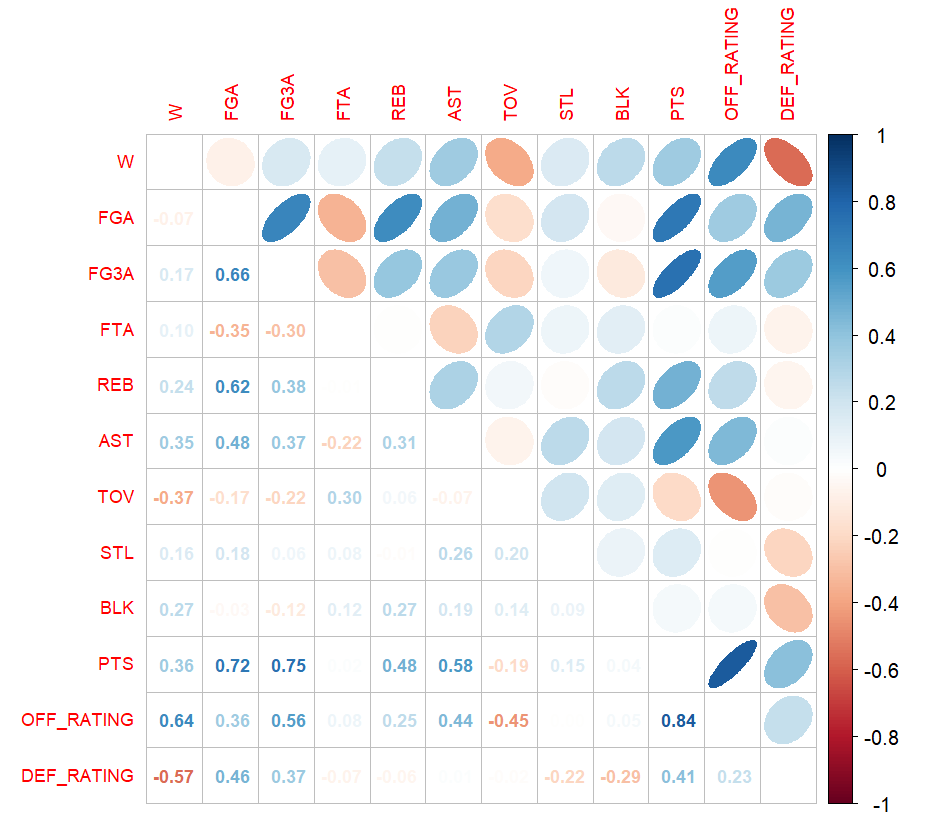
\includegraphics[scale=.5]{imgs/correlation_plot.png}
\end{minipage}
\begin{minipage}{0.5\textwidth} 
    Come è possibile osservare dal grafico riassuntivo delle correlazioni, le vittorie risultano essere nettamente correlate ($+-$ 0.6) con i due indicatori avanzati OFF\_RATING e DEF\_RATING; correlato positivamente con l'OFF\_RATING e negativamente con il DEF\_RATING. Ciò è dovuto alla natura opposta delle due statistiche: vincerà un numero maggiore di partite la squadra che totalizzerà un grande numero di punti, OFF\_RATING elevato, e ne subirà il meno possibile, DEF\_RATING ridotto.
    Le palle perse, gli assist e i punti hanno invece delle correlazioni più lievi (circa |0.35|).
\end{minipage}

\section{Analisi}
Per effettuare l'analisi sono stati confrontati un modello di regressione lineare e un modello di regressione non lineare, logaritmico. Dato il consistente numero di fattori di ingresso, è stata operata una riduzione valutando di volta in volta, i valori di \emph{varianza spiegata}, \emph{varianza spiegata corretta} e i p-value dei fattori di ingresso. 

\subsection{Modello di Regressione Lineare}
Il primo dei due modelli, è stato ottenuto tramite una riduzione in 9 passaggi totali.
Il settimo modello è il primo a presentare dei p-value significativamente bassi e anche un buon valore di $R^2_{Adj}$ confrontato con gli altri modelli. Rappresenta un buon compromesso tra proporzione di varianza spiegata elevata e numero di attributi e, pertanto, è stato selezionato come modello di regressione.

\begin{figure}[h]
	\hspace{-2.30cm}
	\begin{minipage}{.57\textwidth} 
		\begin{lstlisting}[language=bash,basicstyle=\tiny,tabsize=2,frame = single]
> summary(lm.7)
            
Call:
lm(formula = W ~ .-FG3A-BLK-PTS-FTA-STL-REB, data = data)
            
Residuals:
Min      1Q  Median      3Q     Max 
-9.8940 -1.9632 -0.0257  2.0399  7.2707 
            
Coefficients:
Estimate Std. Error t value Pr(>|t|)    
(Intercept) 48.87061    5.69700   8.578  < 2e-16 ***
FGA         -0.10798    0.04829  -2.236  0.02576 *  
AST          0.15593    0.08206   1.900  0.05796 .  
TOV         -0.32933    0.12602  -2.613  0.00922 ** 
OFF_RATING   2.53288    0.04284  59.119  < 2e-16 ***
DEF_RATING  -2.51066    0.04209 -59.647  < 2e-16 ***
---
Signif. codes: 0 *** 0.001 ** 0.01 * 0.05 . 0.1 ' ' 1
            
Residual standard error: 2.91 on 528 degrees of freedom
Multiple R-squared:  0.945,	Adjusted R-squared:  0.9445 
F-statistic:  1814 on 5 and 528 DF,  p-value: < 2.2e-16
    \end{lstlisting}
\end{minipage}
	\begin{minipage}{0.5\textwidth} 
		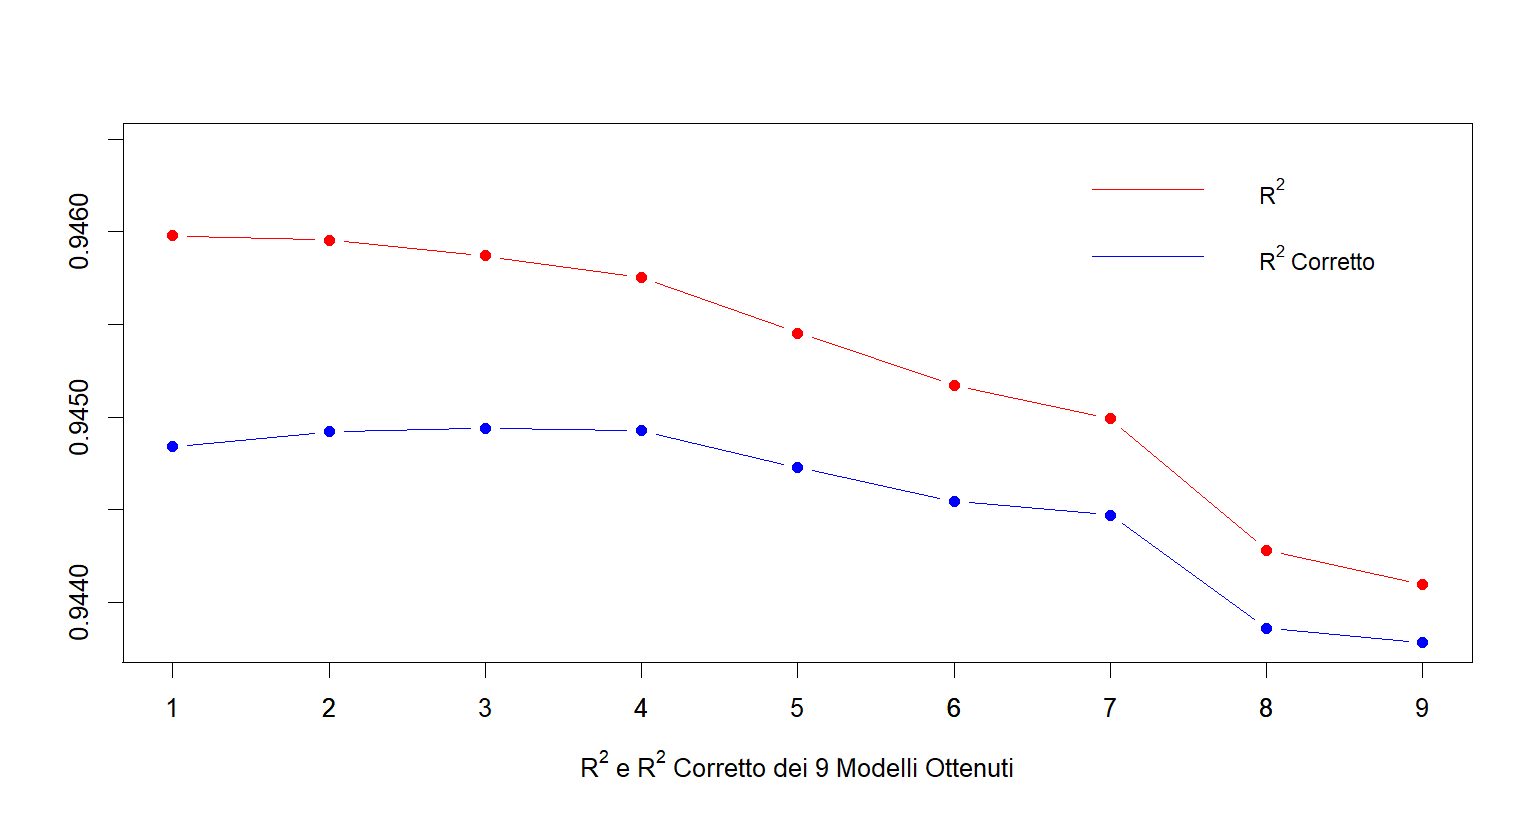
\includegraphics[scale=.45]{imgs/r2_linear_model.png}
	\end{minipage}
\end{figure}

La regressione lineare multivariata basata sul modello risulta avere una proporzione di \emph{varianza spiegata aggiustata} superiore al 94\% e un p-value generale molto basso.

\subsubsection{Analisi dei Residui}
Osservando l'istogramma dei residui, essi appaiono distribuiti normalmente: la distribuzione della densità si avvicina molto a quella di una distribuzione normale, rappresentata nel grafico dalla curva rossa. 
Anche il Q-Q plot ci suggerisce la normalità dei residui, data l'aderenza della quasi totalità dei punti alla bisettrice a meno di qualche outlier.  

\begin{figure}[h]
    \hspace{-1.5cm}
	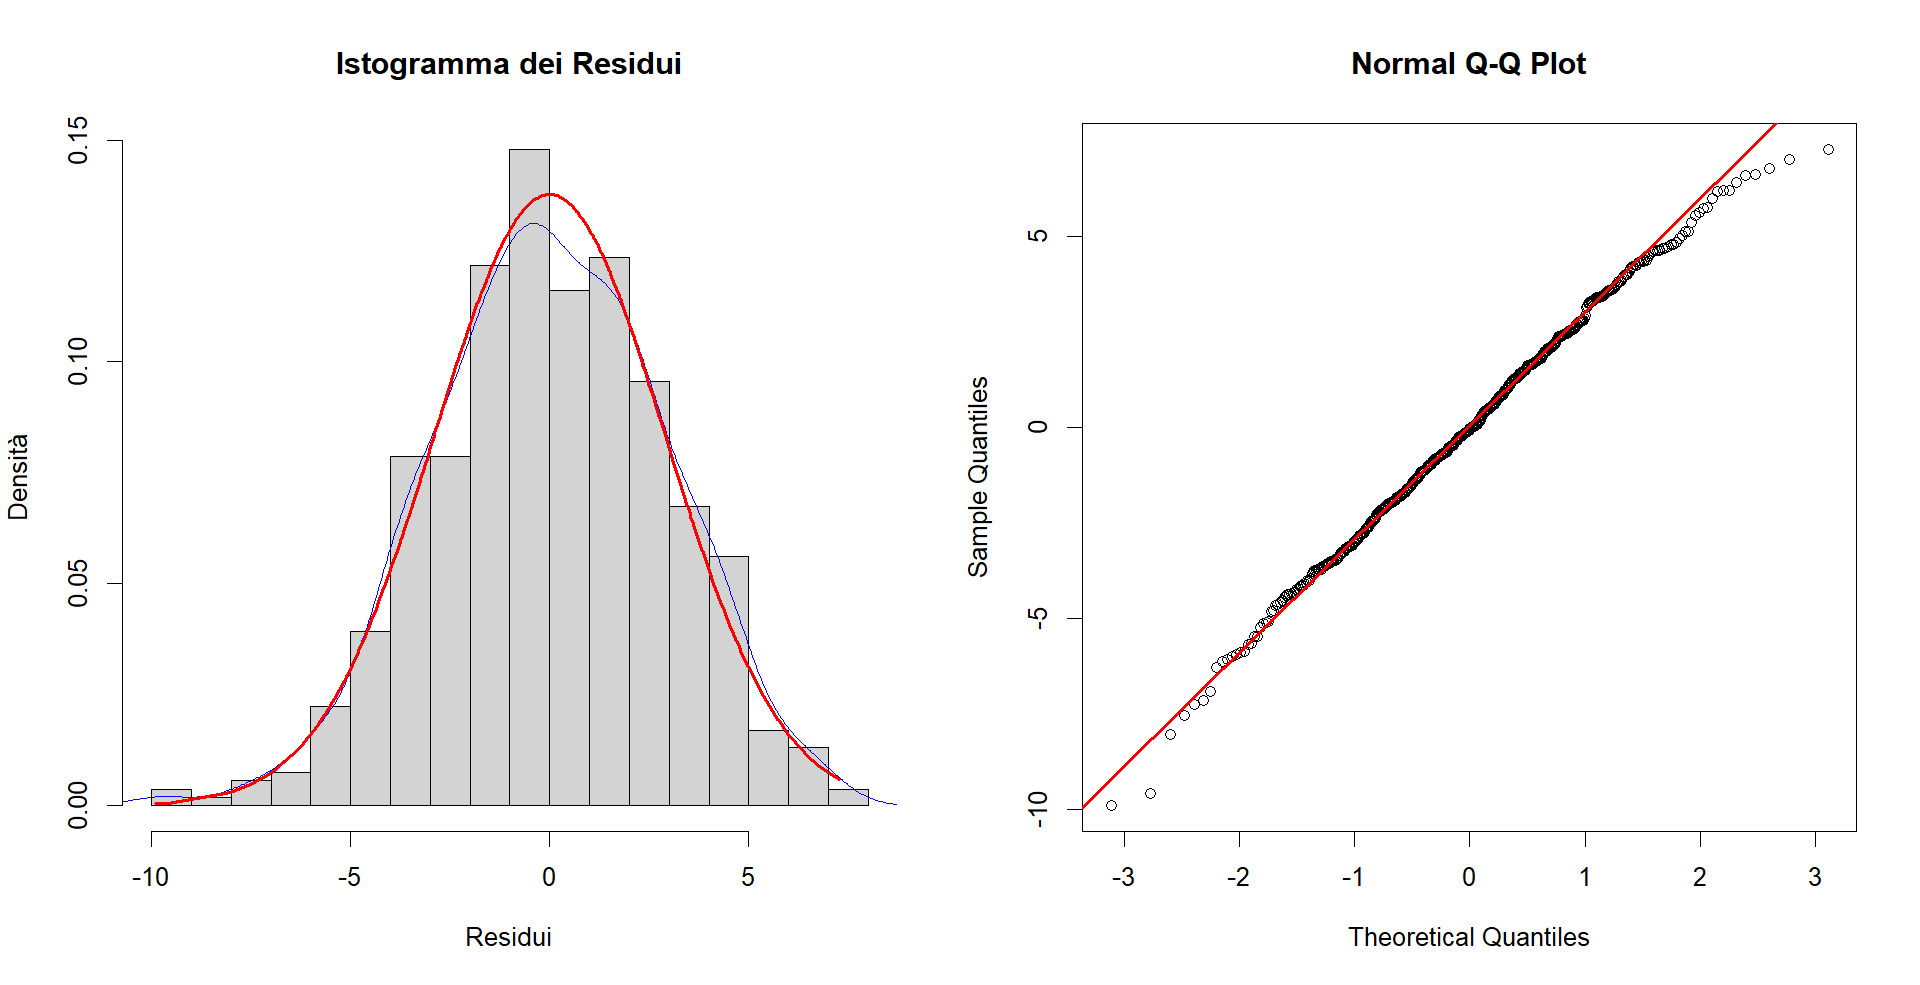
\includegraphics[scale=0.6]{imgs/residuals_analysis_linear_model.png}
    \end{figure}
\vspace{-0.4cm}

\begin{figure}[h]
    \hspace{-2.00cm}
    \begin{minipage}{.6\textwidth} 
    	\begin{lstlisting}[language=bash,basicstyle=\tiny,tabsize=2,frame = single]
> skewness=mean(((lm.r-mean(lm.r))/sd(lm.r))^3)
> skewness
[1] -0.1370172
> kurtosi=mean(((lm.r-mean(lm.r))/sd(lm.r))^4)-3
> kurtosi
[1] -0.07409105
> shapiro.test(lm.r)
        
	Shapiro-Wilk normality test
        
data:  lm.r
W = 0.99671, p-value = 0.3498
        \end{lstlisting}
    \end{minipage}
    \hspace{0.07\textwidth}%
    \begin{minipage}{0.5\textwidth} 
    	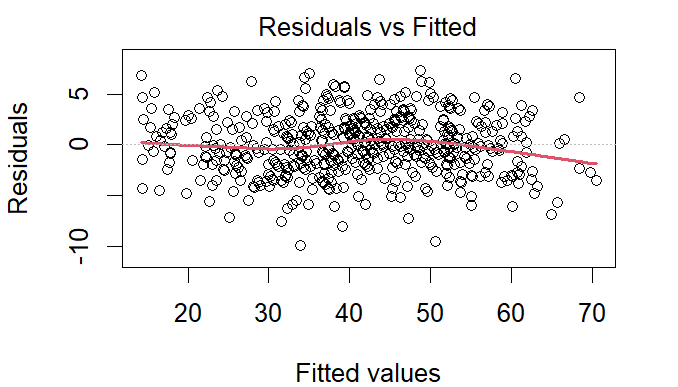
\includegraphics[scale=.45]{imgs/residuals_linear_model.png}
    \end{minipage}
\end{figure}
Osservando il grafico di dispersione dei valori residui e dei valori stimati, si nota come i residui si disperdano in modo simile su tutto il grafico, verosimilmente con varianza omogenea. Anche in questo caso possiamo notare la presenza di outliers, posizionati prevalentemente nella parte centrale-bassa del grafico. La linea rossa, rappresentante la tendenza dei residui, è abbastanza sovrapponibile alla linea tratteggiata, corrispondente dei residui con media zero, allora l’ipotesi di linearità è verificata, ovvero i residui si distribuiscono in modo casuale intorno allo 0.

Skewness e Kurtosi sono entrambi bassi, ulteriore conferma della normalità.

Andando a verificare la normalità dei residui, il test di Shapiro Wilk restituisce un p-value decisamente superiore ai livelli di significatività a cui di solito si fa riferimento (alpha=0.05): ciò impedisce di rigettare l'ipotesi nulla ovvero la normalità della distribuzione.

L'analisi dei residui è stata decisamente positiva, abbiamo la conferma che il modello abbia catturato l'essenza del problema dato che gli errori sembrano dovuti esclusivamente al caso.

\subsection{Modello di Regressione Non Lineare}
Il modello di regressione lineare ha dato ottimi risultati, tuttavia è stato ritenuto necessario andare a verificare se un modello di regressione logaritmico potesse fornire previsioni migliori, magari riuscendo a catturare componenti non lineari del problema. 
Dei nove modelli ottenuti tramite riduzione, questa volta è stato selezionato il nono poiché il primo a presentare p-value sufficientemente bassi.

\begin{figure}[h]
	\hspace{-2.30cm}
    \begin{minipage}{.6\textwidth} 
	\begin{lstlisting}[language=bash,basicstyle=\tiny,tabsize=2,frame = single]
> summary(lm.log)
        
Call:
lm(formula = W ~ .-FG3A-FTA-PTS-BLK-STL-REB-AST-FGA, data = ldata)
        
Residuals:
     Min       1Q   Median       3Q      Max 
-0.61935 -0.05781  0.00720  0.07747  0.25661 
        
Coefficients:
            Estimate Std. Error t value Pr(>|t|)    
(Intercept)  4.10873    0.87219   4.711 3.16e-06 ***
TOV         -0.16678    0.06454  -2.584     0.01 *  
OFF_RATING   7.26847    0.14497  50.137  < 2e-16 ***
DEF_RATING  -7.26919    0.13770 -52.790  < 2e-16 ***
---
Signif. codes:  0 *** 0.001 ** 0.01 * 0.05 . 0.1 ' ' 1
        
Residual standard error: 0.1065 on 530 degrees of freedom
Multiple R-squared:  0.9042,	Adjusted R-squared:  0.9037 
F-statistic:  1668 on 3 and 530 DF,  p-value: < 2.2e-16
	    \end{lstlisting}
    \end{minipage}
	\begin{minipage}{0.5\textwidth} 
		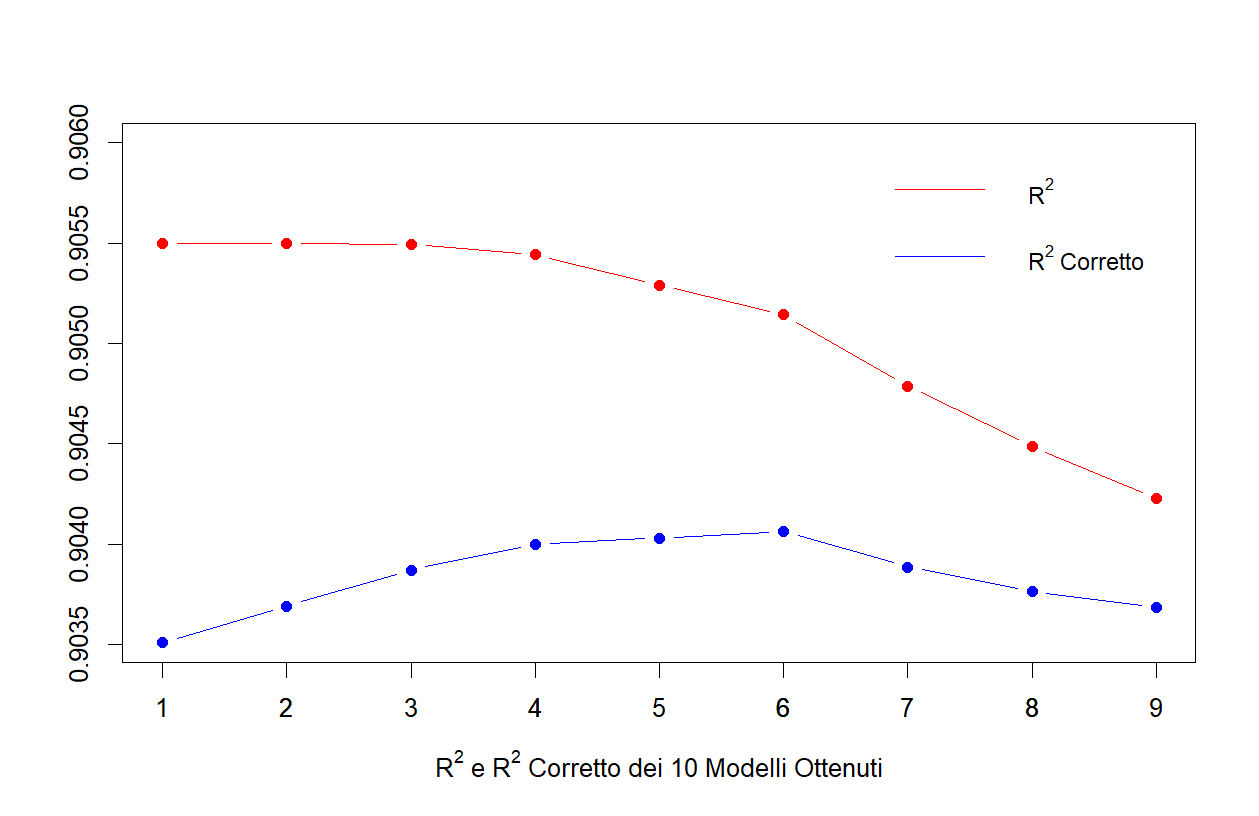
\includegraphics[scale=.53]{imgs/r2_log_model.png}
	\end{minipage}
\end{figure}

Rispetto al modello lineare, la proporzione di varianza spiegata e varianza spiegata aggiustata calano di circa 4.5\% e, inoltre, il modello logaritmico possiede un numero inferiore di fattori di ingresso considerati. Anche in questo modello sono presenti entrambi gli indicatori avanzati di OFF\_RATING e DEF\_RATING, come mostrato nelle considerazioni preliminari, sono i fattori di ingresso più correlati al numero di vittorie.

\subsubsection{Analisi dei Residui}
 L'istogramma dei residui è simile a quello nel caso lineare mentre il Q-Q plot mostra le code della gaussiana discostarsi, anche notevolmente, dalla bisettrice.

\begin{figure}[h]
    \hspace{-1.5cm}
	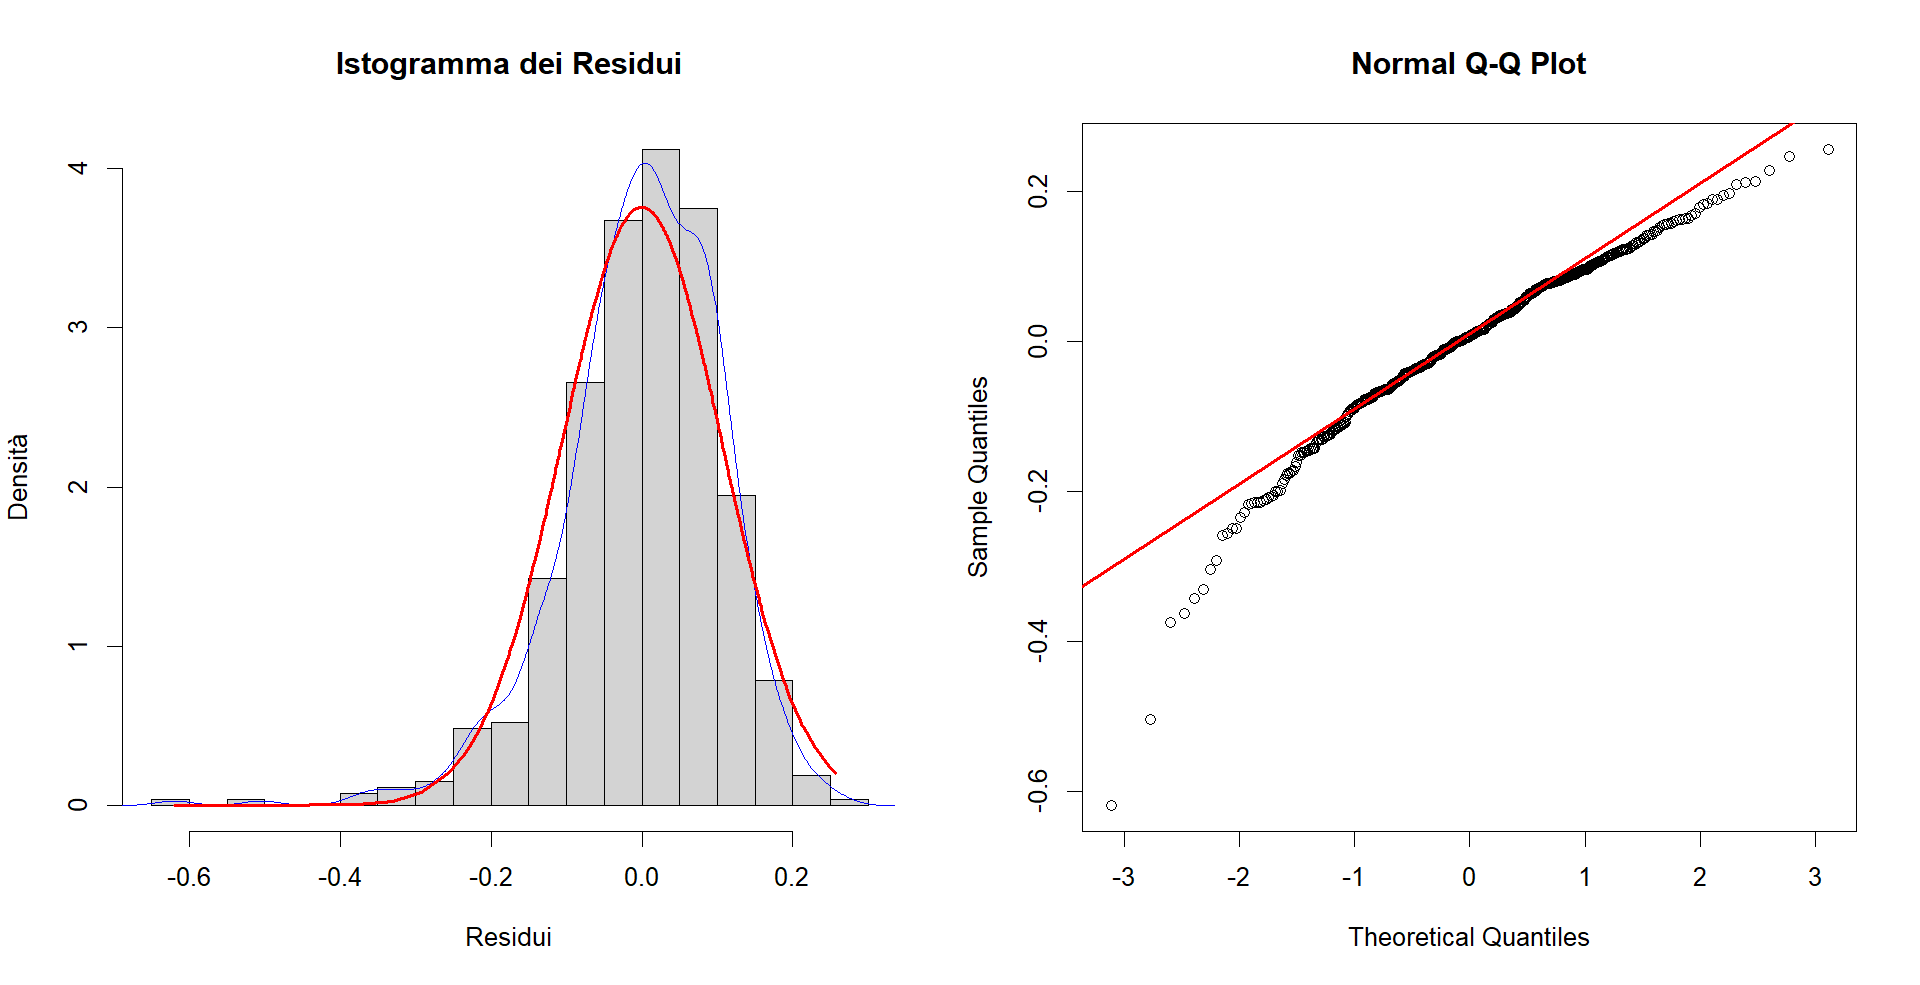
\includegraphics[scale=0.6]{imgs/residuals_analysis_log_model.png}
    \end{figure}
\vspace{-0.4cm}

Il grafico di dispersione dei valori residui e dei valori stimati evidenzia una relazione particolare tra i residui: situazione in cui non c’è linearità suggerisce che il modello logaritmico potrebbe non essere il più adeguato all'analisi del fenomeno.

Nonostante la forte similitudine con il grafico di una distribuzione normale, il test di Shapiro Wilk ha un p-value molto ridotto che costringe a rifiutare l'ipotesi nulla di normalità dei residui.

\begin{figure}[h]
    \hspace{-2.00cm}
    \begin{minipage}{.6\textwidth} 
    	\begin{lstlisting}[language=bash,basicstyle=\tiny,tabsize=2,frame = single]
> skewness=mean(((lm.log.r-mean(lm.log.r))/sd(lm.log.r))^3)
> skewness
[1] -1.009664
> kurtosi=mean(((lm.log.r-mean(lm.log.r))/sd(lm.log.r))^4)-3
> kurtosi
[1] 3.05411
> shapiro.test(lm.log.r)
        
    Shapiro-Wilk normality test
        
data: lm.log.r
W = 0.95504, p-value = 1.101e-11
    	\end{lstlisting}
    \end{minipage}
    \hspace{0.07\textwidth}%
    \begin{minipage}{0.5\textwidth} 
    	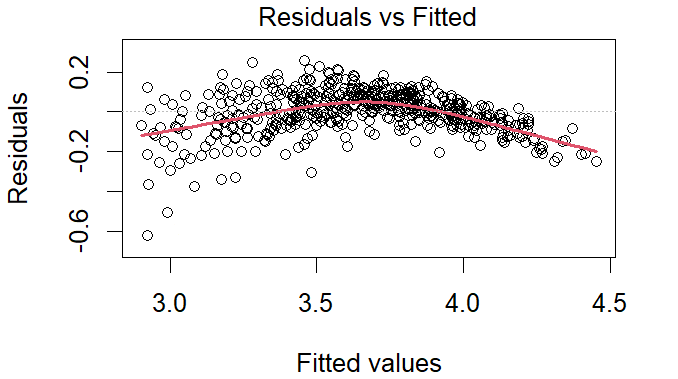
\includegraphics[scale=.45]{imgs/residuals_log_model.png}
    \end{minipage}
\end{figure}

La non normalità potrebbe essere dovuta al processo di riduzione ma, come mostrato in figura, il p-value ottenuto eseguendo il test sul modello non ridotto restituisce risultati circa uguali a quelli del test effettuato sul modello ridotto.
\vspace{0.5cm}
\begin{lstlisting}[language=bash,basicstyle=\tiny,tabsize=2,frame = single]
> # valutazione dei residui del modello di regressione non ridotto
> lm.log.1.r = residuals(lm.log.1)
> shapiro.test(lm.log.1.r)

	Shapiro-Wilk normality test

data:  lm.log.1.r
W = 0.95491, p-value = 1.051e-11
\end{lstlisting}
\vspace{0.5cm}

La non normalità dei residui, allora, potrebbe essere ricondotta alla presenza di outliers che potrebbero avere un'incidenza negativa sul modello (come intuibile dal Q-Q plot).
Si possono ottenere risultati decisamente più soddisfacenti se venissero rimossi gli outliers.

\vspace{0.5cm}
\begin{lstlisting}[language=bash,basicstyle=\tiny,tabsize=2,frame = single]
# rimozione dei residui outliers
r_outliers <- boxplot(lm.log.r, plot=FALSE)$out
r_outliers <- rev(sort(r_outliers))
r_outliers
lm.log.r<-lm.log.r[-which(lm.log.r %in% r_outliers[1:length(r_outliers)])]

\end{lstlisting}

\begin{figure}[h]
    \vspace{-0.3cm}
    \hspace{-2.00cm}
    \begin{minipage}{.6\textwidth} 
    	\begin{lstlisting}[language=bash,basicstyle=\tiny,tabsize=2,frame = single]
> # indicatori post rimozione outliers
> skewness=mean(((lm.log.r-mean(lm.log.r))/sd(lm.log.r))^3)
> skewness
[1] -0.3017812
> kurtosi=mean(((lm.log.r-mean(lm.log.r))/sd(lm.log.r))^4)-3
> kurtosi
[1] -0.05749205
> shapiro.test(lm.log.r)

	Shapiro-Wilk normality test

data:  lm.log.r
W = 0.99107, p-value = 0.002883
    	\end{lstlisting}
    \end{minipage}
    \hspace{0.04\textwidth}%
    \begin{minipage}{0.5\textwidth} 
        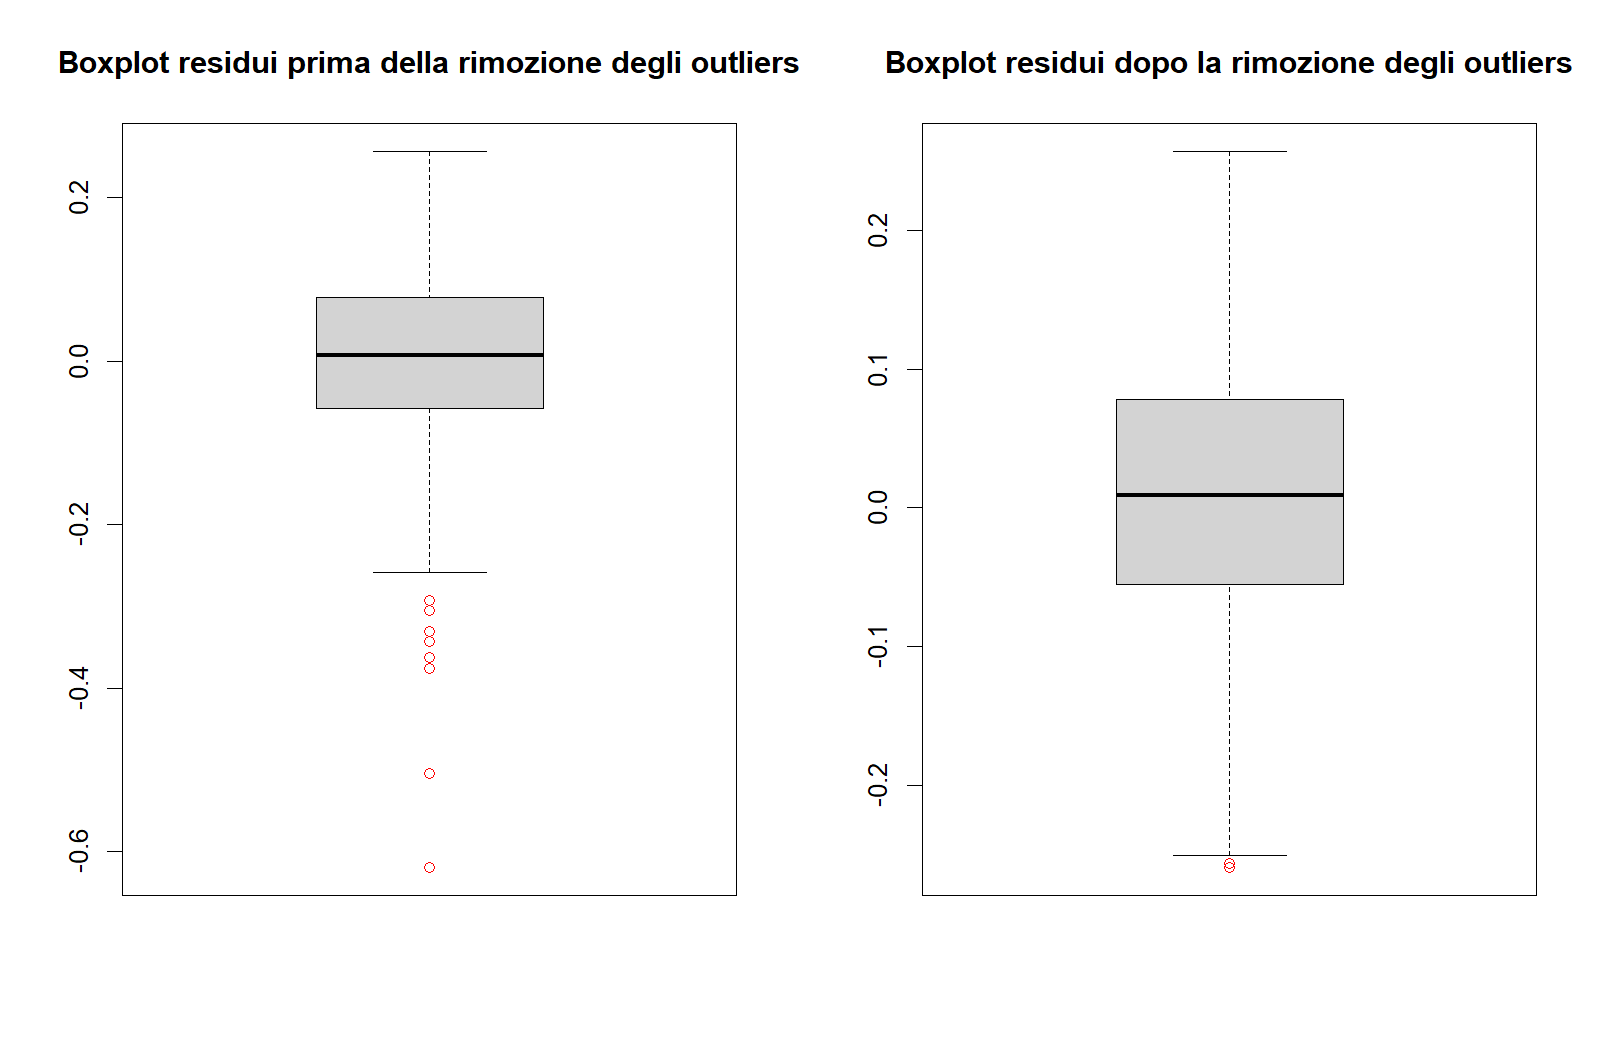
\includegraphics[scale=0.35]{imgs/boxplots_residuals.png}
    \end{minipage}
\end{figure}
\vspace{-1.6cm}

\begin{figure}[h]
    \hspace{-1.5cm}
	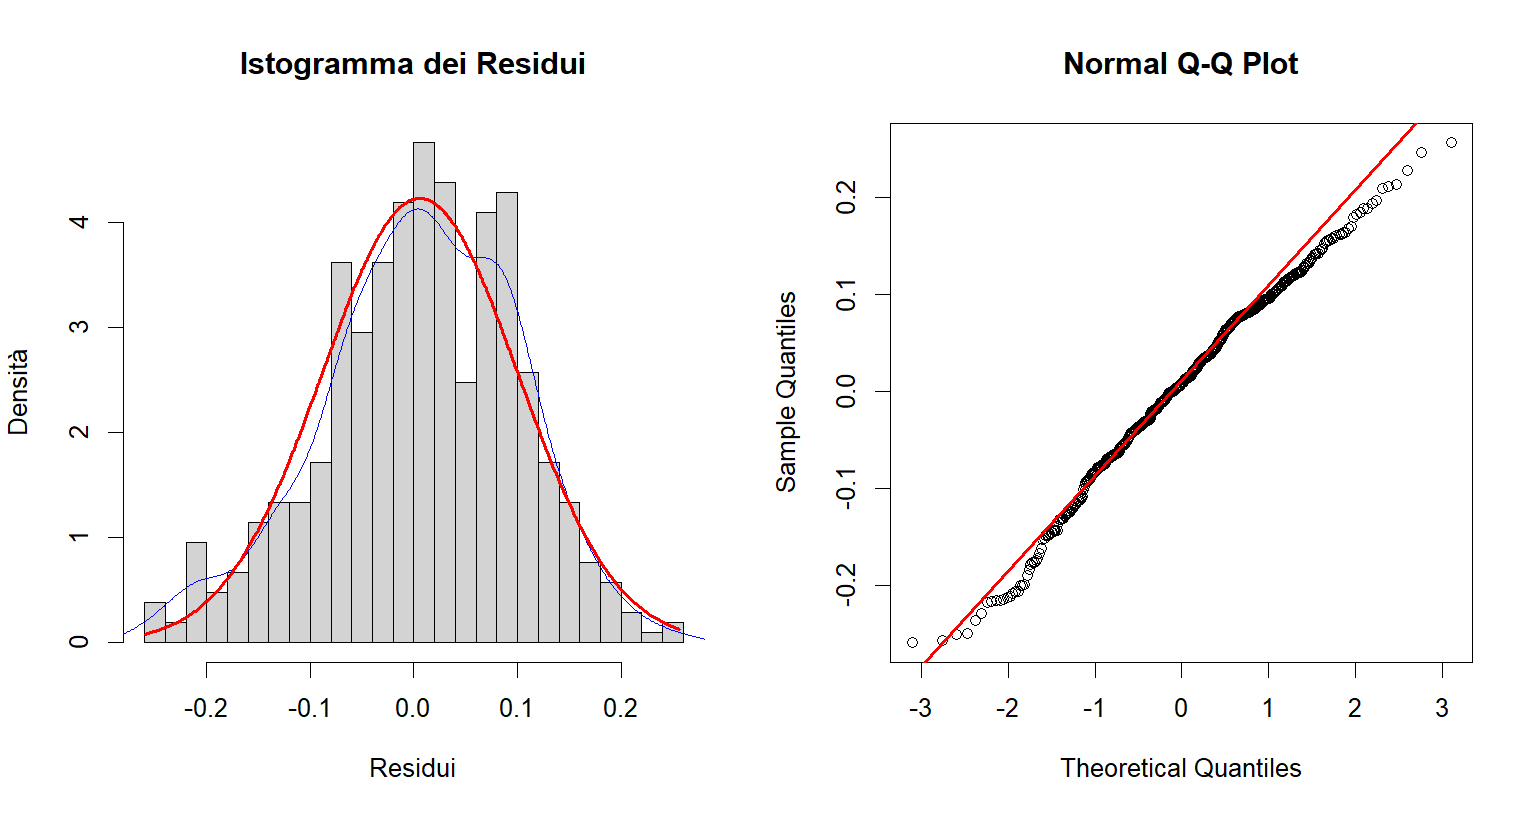
\includegraphics[scale=0.75]{imgs/residuals_analysis_log_model_after_outliers_removals.png}
    \end{figure}
\vspace{-0.4cm}

Dopo la rimozione di 8 outliers, il Q-Q plot mostra i residui molto più aderenti siano sovrapposti alla bisettrice, il valore di skewness e soprattutto di kurtosi sono più piccoli;
il test di Shapiro Wilk restituisce un p-value decisamente migliorato però non permette ancora di rigettare l'ipotesi nulla di normalità.

L'analisi dei residui sul modello non lineare, alla fine, ha dato risultati accettabili, siamo comunque lontani dalla normalità dei residui trovata con il modello lineare.

\section{Previsione e Autovalutazione}
Avendo due modelli con proporzione di varianza spiegata elevata, rispettivamente di 94\% e 90\%, l'analisi dei residui potrebbe non essere sufficiente a distinguere chiaramente quale dei due sia un modello migliore.

Per esprimere un giudizio definitivo sui due modelli analizzati, sono stati messi a confronto: le 534 osservazioni sono state divise in un sottoinsieme di 50, utilizzate come \emph{test set}, e le restanti 484, utilizzate come \emph{training set}.
Questo procedimento è stato ripetuto per un totale di 50 iterazioni in modo da garantire una certa rilevanza statistica.

I risultati delle 50 iterazioni sono riportati nel seguente grafico.

\begin{figure}[H]
	\begin{center}
		\vspace{-0.4cm}
		\hspace*{-2.7cm}
		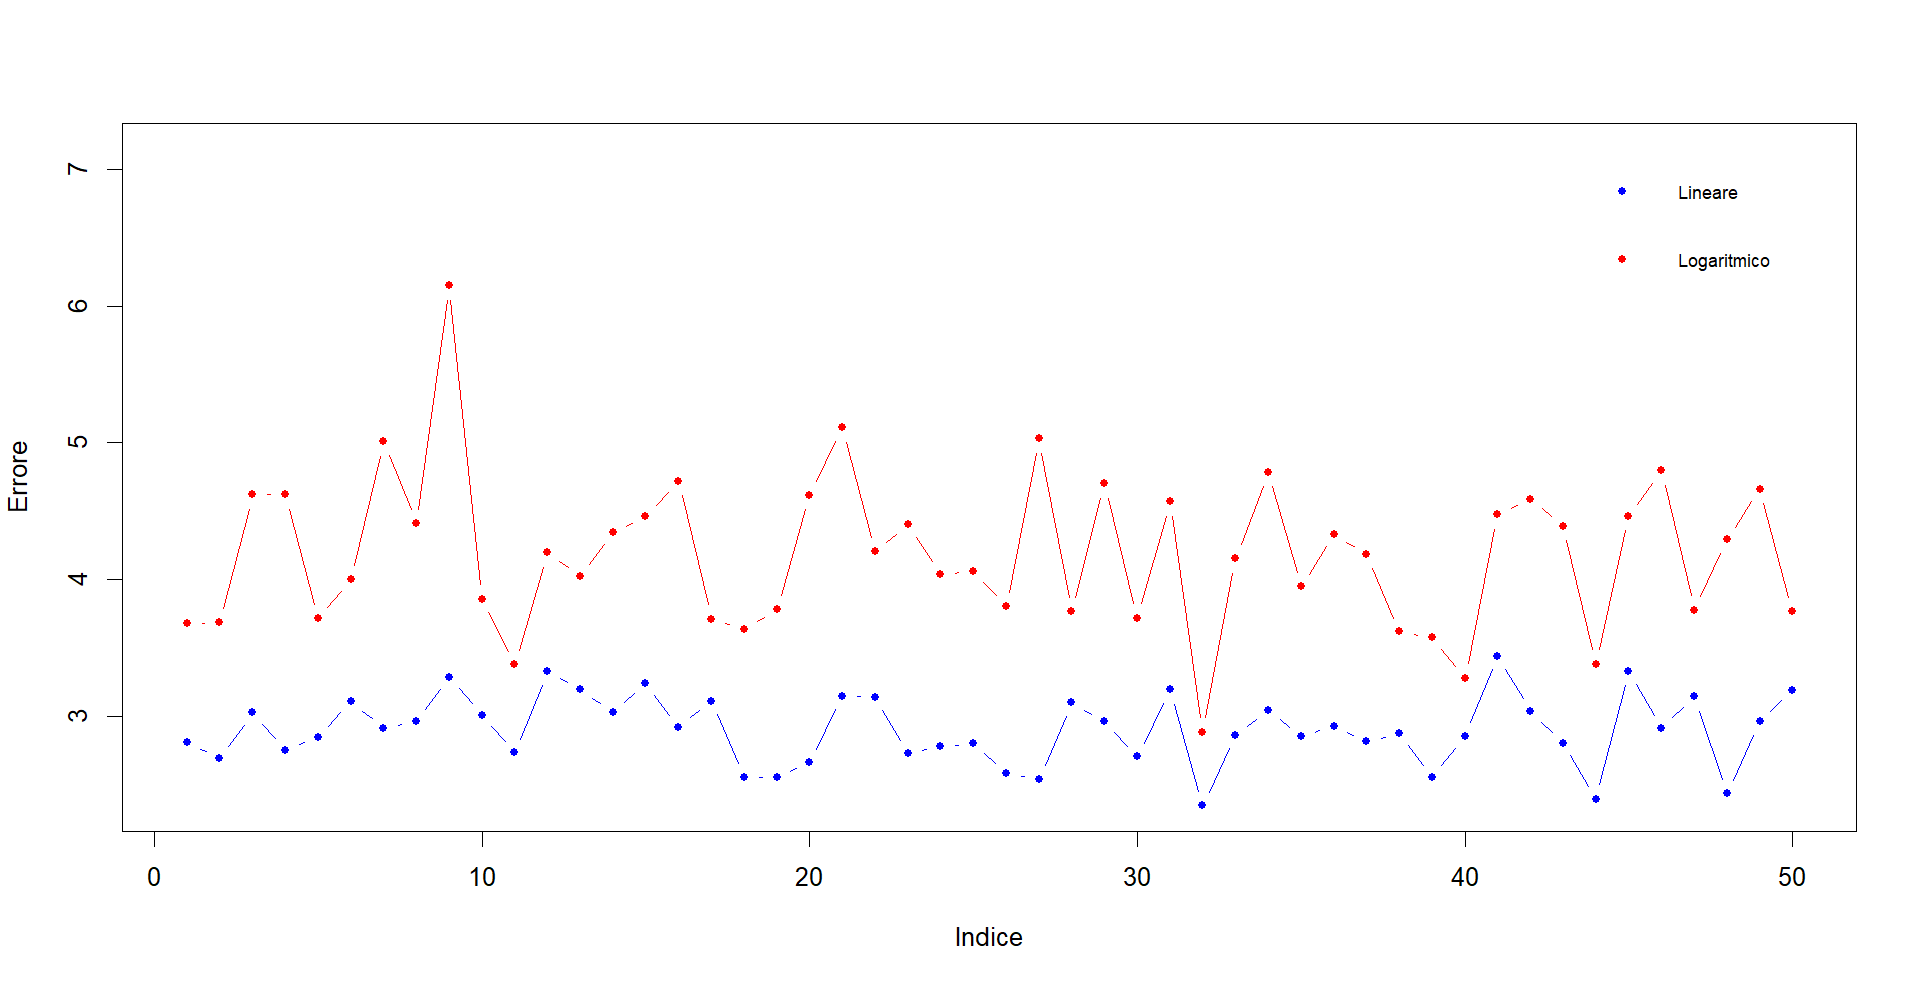
\includegraphics[scale=0.65]{imgs/results.png}
		\vspace{-1.5cm}
	\end{center}
\end{figure}

Come visibile, il modello lineare ha dato risultati migliori: 
ha una media di errore più bassa e una deviazione standard inferiore.

\begin{lstlisting}[language=bash,basicstyle=\tiny,tabsize=2,frame = single]
> # media errori
> mean(err_lin)
[1] 2.903416
> mean(err_log)
[1] 4.1868
> # deviazione standard errori
> sd(err_lin)
[1] 0.2566418
> sd(err_log)
[1] 0.5712424
\end{lstlisting}

\section{Conclusioni}
Innanzitutto, i parametri avanzati selezionati per l'analisi, ovvero OFF\_RATING E DEF\_RATING, si sono rivelati i fattori di ingresso 

In conclusione, il modello lineare è sicuramente quello più affidabile e più adatto al problema. La relazione tra il numero di vittorie e i fattori di ingresso è di tipo lineare, come poteva essere intuito dall'analisi del grafico di dispersione dei valori residui e dei valori stimati nel caso del modello di regressione non lineare.
ANche dalla presenza di outliers che nel caso lineare venivano interpretati correttamente dal modello, mentre nel caso non lineare venivano visti come outliers.

Nonostante questo, il modello di regressione non lineare è un buon modello, che ha come pregio un numero inferiore di fattori di ingresso ma che risulta essere anche meno preciso di quello lineare.

\newpage
\appendix
\section{Appendice}
 Lo script utilizzato per ottenere le due tabelle utilizzate nell'analisi, fa uso delle \emph{nba-api} ufficiali per Python.
 La funzione \emph{get\_data()}, per ogni stagione indicata nella lista "seasons", scarica i dati sotto forma di liste di \emph{dictonaries} utilizzando la funzione \emph{leaguedashteamstats\.LeagueDashTeamStats} delle \emph{nba-api}. Specificando il valore "Base" del parametro \emph{measure\_type\_detailed\_defense} sarà possibile scaricare le informazioni della tabella \emph{Teams General Traditional}; specificando invece il valore "Advanced" le informazioni saranno quelle della tabella \emph{Teams General Advanced}.
 
 Una volta ottenute entrambe le liste di \emph{dictionaries}, \emph{get\_data()} le unisce usando il codice seguente e le aggiunge al dataframe da restituire.

\vspace{0.5cm} 
\begin{lstlisting}[language=python,tabsize=1,frame = single]
d = defaultdict(dict)
for l in (allTeamsTraditionalList, allTeamsAdvancedList):
    for elem in l:
        d[elem['TEAM_ID']].update(elem)
result = d.values()
\end{lstlisting}
\vspace{0.5cm}
 
Dal dataframe ottenuto tramite \emph{get\_data()}, vengono rimosse tutte le informazioni che non sono presenti nelle tabelle ai link riportati in precedenza. In particolare le colonne contenenti i ranking relativi ai vari aspetti del gioco (PTS\_RANK, AST\_RANK). Infine, il dataframe viene salvato in formato .csv con il nome "tabella.csv".
\end{document}